\newcommand{\NWtarget}[2]{#2}
\newcommand{\NWlink}[2]{#2}
\newcommand{\NWtxtMacroDefBy}{Fragment defined by}
\newcommand{\NWtxtMacroRefIn}{Fragment referenced in}
\newcommand{\NWtxtMacroNoRef}{Fragment never referenced}
\newcommand{\NWtxtDefBy}{Defined by}
\newcommand{\NWtxtRefIn}{Referenced in}
\newcommand{\NWtxtNoRef}{Not referenced}
\newcommand{\NWtxtFileDefBy}{File defined by}
\newcommand{\NWtxtIdentsUsed}{Uses:}
\newcommand{\NWtxtIdentsNotUsed}{Never used}
\newcommand{\NWtxtIdentsDefed}{Defines:}
\newcommand{\NWsep}{${\diamond}$}
\newcommand{\NWnotglobal}{(not defined globally)}
\newcommand{\NWuseHyperlinks}{}
\documentclass{article}
\usepackage{graphicx}
\usepackage{hyperref}
\usepackage{tikz}
\title{P3.24}
\author{Frank Mock}
\begin{document}
\maketitle
\section{Specification}
Exercise P3.24.      
Write a program that draws a square with corner points (0, 0) and (1, 1). 
Prompt the user for a mouse click. If the user clicked inside the square, 
then show a message Congratulations. Otherwise, show a message You missed. 
\section{Design}
Assume that the points forming the square have dimensions:\\
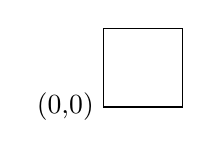
\begin{tikzpicture}
\draw(0,0) rectangle(1,1);
\draw(0,0) node[anchor=east]{(0,0)};
\end{tikzpicture}\\
and that the user's point is in variable $p$.
Display the message to the user someplace outside the square. For
example at some point (2,2).
\section{Implementation}

\begin{flushleft} \small
\begin{minipage}{\linewidth}\label{scrap1}\raggedright\small
\NWtarget{nuweb1}{} \verb@"p3_24.cpp"@\nobreak\ {\footnotesize {1}}$\equiv$
\vspace{-1ex}
\begin{list}{}{} \item
\mbox{}\verb@@\\
\mbox{}\verb@@\hbox{$\langle\,${\it Include Files}\nobreak\ {\footnotesize \NWlink{nuweb3c}{3c}}$\,\rangle$}\verb@@\\
\mbox{}\verb@int ccc_win_main()//authors entry point that calls name@\\
\mbox{}\verb@{@\\
\mbox{}\verb@@\hbox{$\langle\,${\it Draw a Square}\nobreak\ {\footnotesize \NWlink{nuweb2a}{2a}}$\,\rangle$}\verb@@\\
\mbox{}\verb@@\hbox{$\langle\,${\it Get the point where the user clicked}\nobreak\ {\footnotesize \NWlink{nuweb2b}{2b}}$\,\rangle$}\verb@@\\
\mbox{}\verb@@\hbox{$\langle\,${\it Determine if that point is in the square}\nobreak\ {\footnotesize \NWlink{nuweb3a}{3a}}$\,\rangle$}\verb@@\\
\mbox{}\verb@return 0;@\\
\mbox{}\verb@}@\\
\mbox{}\verb@@{\NWsep}
\end{list}
\vspace{-1.5ex}
\footnotesize
\begin{list}{}{\setlength{\itemsep}{-\parsep}\setlength{\itemindent}{-\leftmargin}}

\item{}
\end{list}
\end{minipage}\vspace{4ex}
\end{flushleft}
The authors graphics library includes a \verb|Point| class and
a \verb|Line| class which allow points and lines to be drawn on
the screen. A \verb|Point| has an \verb|x-| and a \verb|y-coordinate.|
For example, \verb|Point(1,3)| is a \verb|Point| with \verb|x-coordinate|
1 and \verb|y-coordinate| 3. Two points can be joined by a line, represented
by a \verb|Line| object that is contructed from two \verb|Point| objects,
it's start point and end points.\\
\indent \verb|Point p(1, 3);|\\
\indent \verb|Point q(4, 7);|\\
\indent \verb|Line s(p, q);|\\
Both the \verb|Point| and \verb|Line| class implement the member function
\verb|move(x, y)| which changes position of an object, moving the entire
object by the \verb|x| and \verb|y| units specified.\\
\indent \verb|s.move(1, 0)|\\
This moves the line \verb|s| 1 unit in the x direction (to the right). cwin
is a window object used to display graphic objects such as \verb|Line| and
\verb|Point| to the screen.\\
\indent \verb|cwin << s;|\\
\begin{flushleft} \small
\begin{minipage}{\linewidth}\label{scrap2}\raggedright\small
\NWtarget{nuweb2a}{} $\langle\,${\it Draw a Square}\nobreak\ {\footnotesize {2a}}$\,\rangle\equiv$
\vspace{-1ex}
\begin{list}{}{} \item
\mbox{}\verb@@\\
\mbox{}\verb@//draw a 1x1 unit square@\\
\mbox{}\verb@Point top_left(0, 1);@\\
\mbox{}\verb@Point top_right(1, 1);@\\
\mbox{}\verb@Point bottom_left(0, 0);@\\
\mbox{}\verb@        @\\
\mbox{}\verb@Line horizontal(top_left, top_right);@\\
\mbox{}\verb@Line vertical(top_left, bottom_left);@\\
\mbox{}\verb@        @\\
\mbox{}\verb@cwin << horizontal << vertical;@\\
\mbox{}\verb@        @\\
\mbox{}\verb@horizontal.move(0, -1);@\\
\mbox{}\verb@vertical.move(1, 0);@\\
\mbox{}\verb@        @\\
\mbox{}\verb@cwin << horizontal << vertical;@\\
\mbox{}\verb@@{\NWsep}
\end{list}
\vspace{-1.5ex}
\footnotesize
\begin{list}{}{\setlength{\itemsep}{-\parsep}\setlength{\itemindent}{-\leftmargin}}
\item \NWtxtMacroRefIn\ \NWlink{nuweb1}{1}.

\item{}
\end{list}
\end{minipage}\vspace{4ex}
\end{flushleft}
In the author's library, there is a function named \verb|get_mouse| that
returns the point where the left-button of the mouse was clicked. Invoke it
using the \verb|cwin| object. Store the point in variable \verb|p|
\begin{flushleft} \small
\begin{minipage}{\linewidth}\label{scrap3}\raggedright\small
\NWtarget{nuweb2b}{} $\langle\,${\it Get the point where the user clicked}\nobreak\ {\footnotesize {2b}}$\,\rangle\equiv$
\vspace{-1ex}
\begin{list}{}{} \item
\mbox{}\verb@@\\
\mbox{}\verb@Point p = cwin.get_mouse("Try to click inside the square.");@\\
\mbox{}\verb@@{\NWsep}
\end{list}
\vspace{-1.5ex}
\footnotesize
\begin{list}{}{\setlength{\itemsep}{-\parsep}\setlength{\itemindent}{-\leftmargin}}
\item \NWtxtMacroRefIn\ \NWlink{nuweb1}{1}.

\item{}
\end{list}
\end{minipage}\vspace{4ex}
\end{flushleft}
There is a member function namedverb|get_x()| and \verb|get_y()| to retrieve
the coordinates from a point object. (e.g. \verb|p|). Compare those coordinates
to the boundries of the square.
\begin{flushleft} \small
\begin{minipage}{\linewidth}\label{scrap4}\raggedright\small
\NWtarget{nuweb3a}{} $\langle\,${\it Determine if that point is in the square}\nobreak\ {\footnotesize {3a}}$\,\rangle\equiv$
\vspace{-1ex}
\begin{list}{}{} \item
\mbox{}\verb@@\\
\mbox{}\verb@//assign x and y coordinates to double variable@\\
\mbox{}\verb@double x = p.get_x();@\\
\mbox{}\verb@double y = p.get_y();@\\
\mbox{}\verb@//determine if the user clciked inside the square@\\
\mbox{}\verb@if(x <= 1 && x >= 0 && y <=1 && y >= 0)@\\
\mbox{}\verb@{@\\
\mbox{}\verb@ cwin << p << Message(p, "Congratulations, You did it!");@\\
\mbox{}\verb@}@\\
\mbox{}\verb@else@\\
\mbox{}\verb@{@\\
\mbox{}\verb@ cwin << p << Message(p, "Sorry, You missed!");@\\
\mbox{}\verb@}@\\
\mbox{}\verb@@{\NWsep}
\end{list}
\vspace{-1.5ex}
\footnotesize
\begin{list}{}{\setlength{\itemsep}{-\parsep}\setlength{\itemindent}{-\leftmargin}}
\item \NWtxtMacroRefIn\ \NWlink{nuweb1}{1}.

\item{}
\end{list}
\end{minipage}\vspace{4ex}
\end{flushleft}
\begin{flushleft} \small
\begin{minipage}{\linewidth}\label{scrap5}\raggedright\small
\NWtarget{nuweb3b}{} \verb@"p3_24.bat"@\nobreak\ {\footnotesize {3b}}$\equiv$
\vspace{-1ex}
\begin{list}{}{} \item
\mbox{}\verb@@\\
\mbox{}\verb@g++ -mwindows -I C:\C++_Programs\bigc2_sourcecode\cccfiles -o p3_24 p3_24.cpp ^@\\
\mbox{}\verb@C:\C++_Programs\bigc2_sourcecode\cccfiles\ccc_msw.cpp ^@\\
\mbox{}\verb@C:\C++_Programs\bigc2_sourcecode\cccfiles\ccc_shap.cpp ^@\\
\mbox{}\verb@-lgdi32@\\
\mbox{}\verb@@{\NWsep}
\end{list}
\vspace{-1.5ex}
\footnotesize
\begin{list}{}{\setlength{\itemsep}{-\parsep}\setlength{\itemindent}{-\leftmargin}}

\item{}
\end{list}
\end{minipage}\vspace{4ex}
\end{flushleft}
Theses are the include files for this program
\begin{flushleft} \small
\begin{minipage}{\linewidth}\label{scrap6}\raggedright\small
\NWtarget{nuweb3c}{} $\langle\,${\it Include Files}\nobreak\ {\footnotesize {3c}}$\,\rangle\equiv$
\vspace{-1ex}
\begin{list}{}{} \item
\mbox{}\verb@@\\
\mbox{}\verb@#include "ccc_win.h"@\\
\mbox{}\verb@@{\NWsep}
\end{list}
\vspace{-1.5ex}
\footnotesize
\begin{list}{}{\setlength{\itemsep}{-\parsep}\setlength{\itemindent}{-\leftmargin}}
\item \NWtxtMacroRefIn\ \NWlink{nuweb1}{1}.

\item{}
\end{list}
\end{minipage}\vspace{4ex}
\end{flushleft}
\section{Test}
\end{document}